% ============================================== %

%%%%%%%%%%%%%%%%%%%%%%%%%%%%%%%%%%%%%%%%%%%%%%%%%%
%%%			  02 Trabalho Prático 02		   %%%
%%%%%%%%%%%%%%%%%%%%%%%%%%%%%%%%%%%%%%%%%%%%%%%%%%

% ============================================== %

\section{Trabalho Prático 02}


Uma barra rígida biapoiada possui apoio elástico de translação no topo. Pede-se traçar os
gráficos de força aplicada ($P$) \textit{versus} deslocamento horizontal
($\delta_\mathrm{H}$) e vertical ($\delta_\mathrm{V}$)  referentes ao ponto de aplicação
da força. Adotar:

$$
\left\{\begin{array}{lcl}
	k_\text{mola} &=& 1\:\:\text{kN/cm} \\
	L &=& 100\:\:\text{cm} \\
	\Delta\theta &=& \frac{\pi}{90}\:\:\text{rad} \\
\end{array}\right.
$$

\begin{figure}[H]
	\centering
	\caption{Sistema estrutural do Trabalho Prático 02.}
	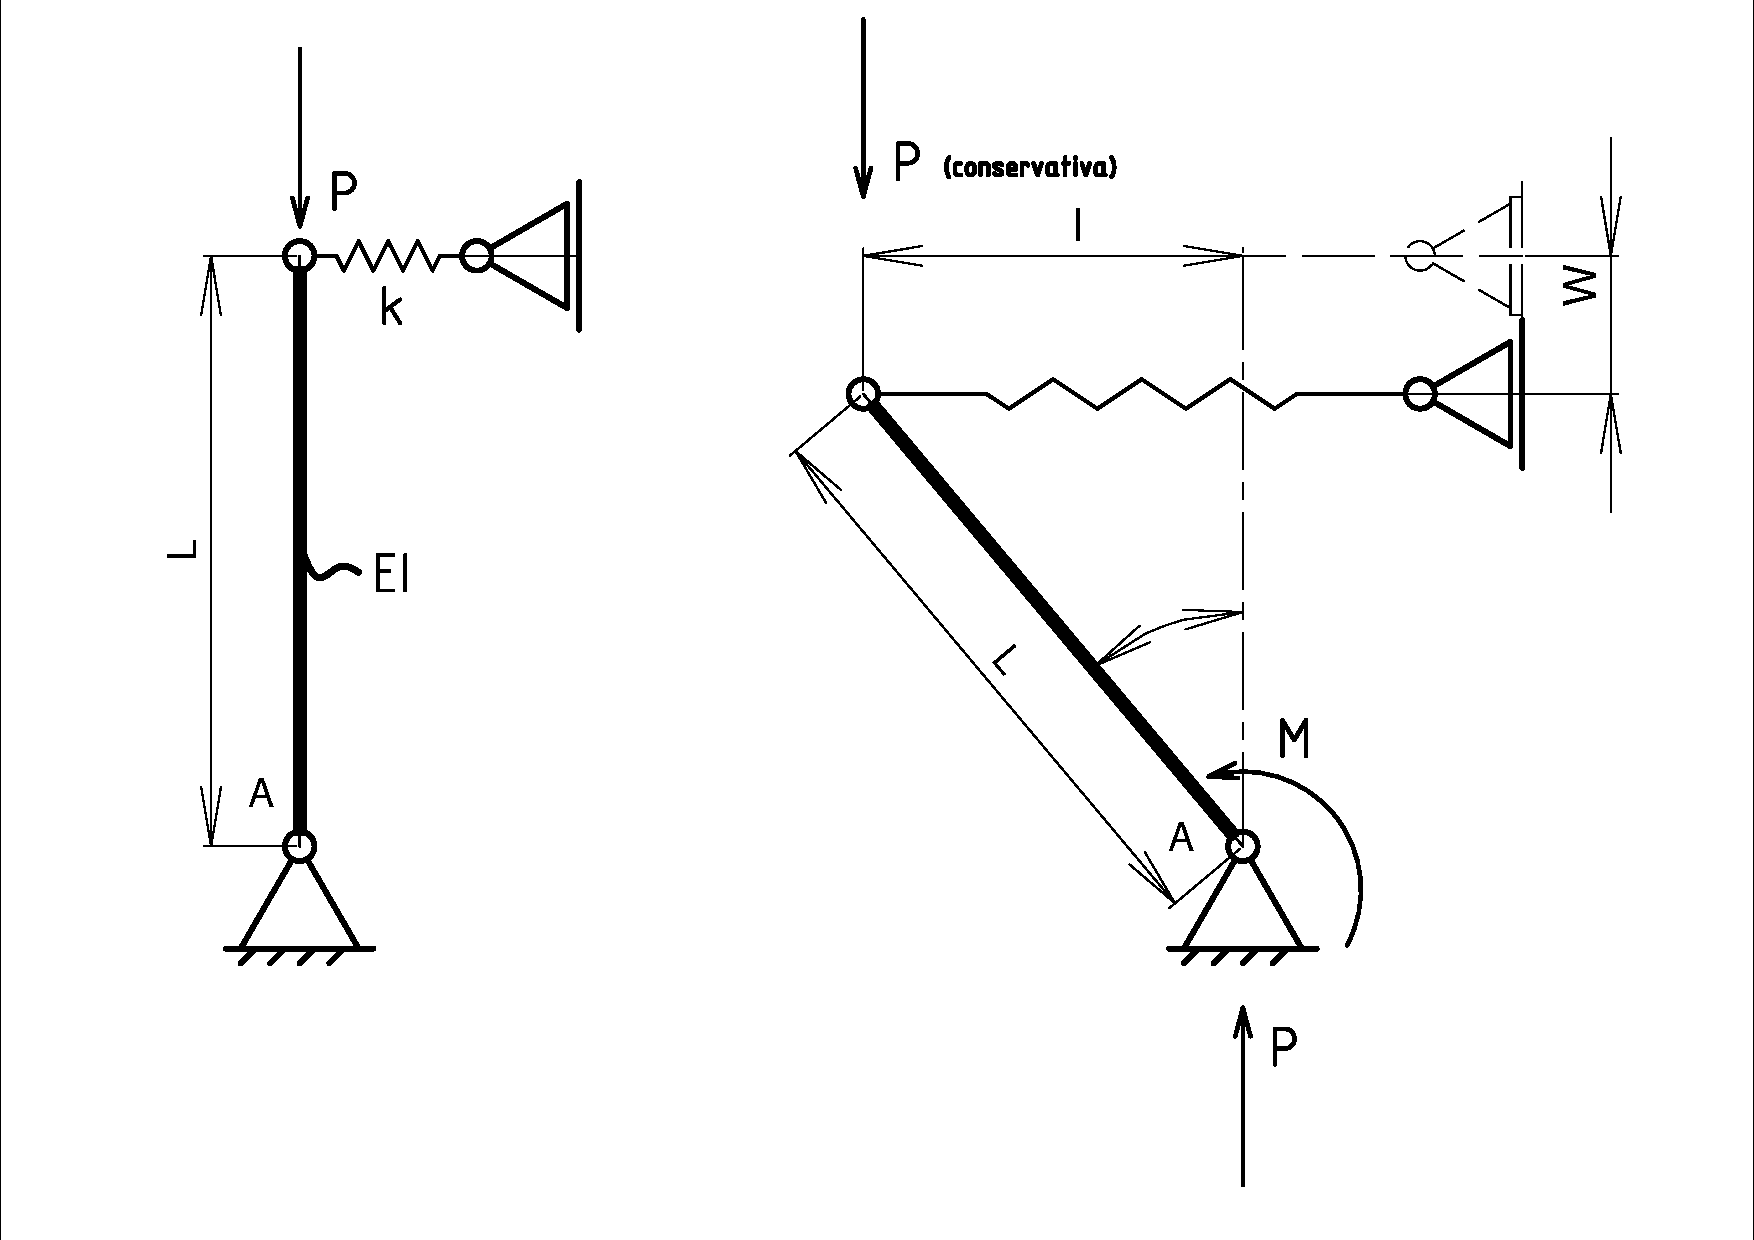
\includegraphics[
		trim=25mm 8mm 2mm 3mm,
		clip,
		width=\textwidth
	]{figuras/TPs-2.pdf}
	\label{fig:TP2}
\end{figure}


% ================ Resolução TP-02 ================
\begin{textocaixa}
\hspace{10mm}

Neste sistema estrutural, assume-se, novamente, \underline{relação constitutiva} linear da
mola:

\begin{equation}
	F_\text{mola} = k_\text{mola}\cdot \delta_h
	\label{eq:TP2-const}
\end{equation}

E como \underline{relações cinemáticas}, tem-se a associação entre as variações $\delta_h$
e $\delta_v$ com o ângulo de giro $\theta$ da barra por meio da \autoref{eq:TP2-cinem}.

\begin{equation}
	\left\{\begin{array}{lcl}
		\delta_h &=& L\sin \theta \\
		\delta_v &=& L\left(1 - \cos\theta\right) \\
	\end{array}\right.
	\label{eq:TP2-cinem}
\end{equation}

Assim, o equilíbrio de momentos em relação ao apoio fixo A resultam na carga $P$ em função do
ângulo $\theta$ dado na \autoref{eq:TP2-P_theta}, assumindo grandes deslocamentos.

\begin{equation}
	P = k_\text{mola}\,L\cdot \cos\theta
	\label{eq:TP2-P_theta}
\end{equation}

Graficamente, essa relação não-linear é expressa pelas curvas $P\times \delta_v$ e
$P\times \delta_h$ mostradas na \autoref{fig:TP2-result}, geradas pelo código dado em
\autoref{subapendice:TP02}.

\begin{figure}[H]
	\centering
	\caption{TP02 $-$ Curvas do carregamento vertical $P$.}
	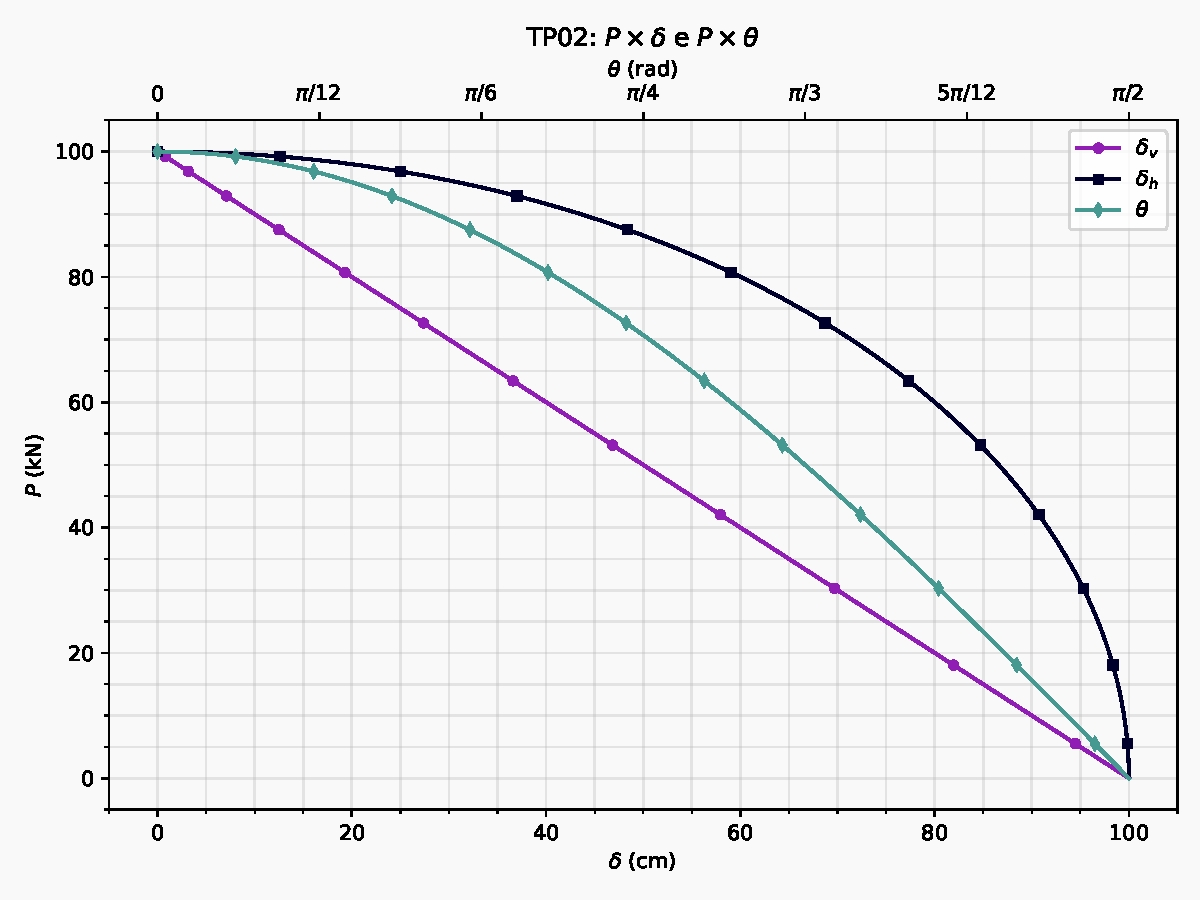
\includegraphics[
		width=\textwidth
	]{figuras/resultados/TP02-result.pdf}
	\label{fig:TP2-result}
\end{figure}

Nesse sistema estrutural, a carga crítica se relaciona com as constantes do problema da
seguinte forma:

\begin{equation}
	P_{cr} = \lim_{\theta\:\longrightarrow\:0} k_\text{mola}\,L\cdot \cos\theta
	\Longrightarrow \boxed{P_{cr} = k_\text{mola}\,L}
	\label{eq:TP2-P_cr}
\end{equation}



\end{textocaixa}